\documentclass{article}

\usepackage{graphicx}
\usepackage[hidelinks]{hyperref}
\usepackage[a4paper, total={6in, 8in}]{geometry}
\usepackage[slovak]{babel}
\usepackage{caption}
\usepackage{subcaption}

\graphicspath{./include/}

\renewcommand{\figurename}{Obr.}
\renewcommand{\contentsname}{Obsah}

\begin{document}

\begin{titlepage}
	\null\vfill

	\begin{center}
		{\Huge Identifikacia servosystemu }
		\vskip 2cm

		{\Large Cvičenie č. 7}
		\vskip 0.5cm

		{\large Spojité procesy}
	\end{center}

	\vfill
	\vfill

	\begin{flushright}
		Filip Lobpreis \\
		Matúš Machata \\
		\small\today\\
	\end{flushright}
	\hfill
\end{titlepage}

\thispagestyle{empty}
\clearpage

\tableofcontents
\thispagestyle{empty}
\clearpage

\section{Zadanie}
\label{sec:zadanie}
\pagenumbering{arabic}

\begin{figure}[!htbp]
	\begin{center}
		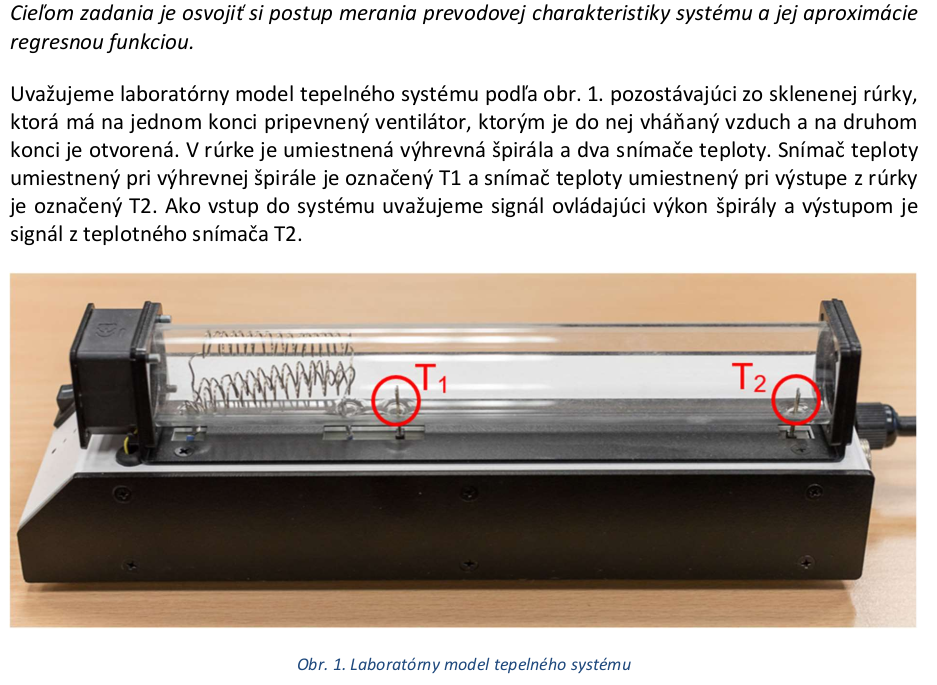
\includegraphics[width=0.8\textwidth]{./include/zadanie.png}
	\end{center}
	\caption{Prvá časť zadania z~cvičenia č. 11 z~predmetu spojité procesy}
	\label{fig:zadanie1}
\end{figure}

\clearpage

\section{Teória}
\label{sec:teoria}

\clearpage

\subsection{Úvod do~priebehu simulácie}
\label{subsec:priebehSimulacie}

\clearpage

\section{Zhrnutie}
\label{sec:zhrnutie}

\end{document}

